% Cluster B: motivating obstructions (manuscript Theorem 6.12, Section 6.4, Proposition 6.15)
% Body-only LaTeX; preamble macros and theorem environments per CONVENTIONS.md.

\section{Obstructions to naive carriers}\label{sec:obstructions}

Before any positive theory is developed, it is worth recording exactly why the
two most tempting shortcuts fail. The first shortcut is a \emph{selection}
rule: given the finite package of marked continua that a carrier must contain,
simply take the least compact connected full set containing it. The second is
a \emph{completion} rule: given a proposed carrier and the excess produced by
pulling it back through the dynamics, simply absorb that excess monotonically
until the process stabilizes. Both rules are natural, both are implicit in
informal uses of connected hulls, and both fail --- the first because the
minimizer does not exist, the second because absorption destroys precisely the
access data that a protected carrier is supposed to preserve. The two
obstructions below are taken from the source manuscript
\cite[Theorem~6.12, Proposition~6.15]{MWman}; they are elementary, but they
dictate the architecture of everything that follows, and in particular the
certificate formalism of Section~\ref{sec:certificates}. The comparison with
standard continuum-hull constructions in Section~\ref{sec:comparison} should
be read with both examples in mind.

\subsection{Failure of least carriers}\label{subsec:B-no-least}

Recall from Section~\ref{sec:prelim} that a compact set $K\subset\C$ is
\emph{full} if $\C\setminus K$ is connected, and that a \emph{carrier} for a
finite package $S\subset\C$ is a compact connected full continuum containing
$S$. Order the carriers of a fixed package by inclusion. A \emph{least}
carrier would be a carrier contained in every other carrier of the same
package. The following theorem shows that a least carrier fails to exist
already for the simplest nontrivial package: two points, with the identity
map as dynamics and with no obstacle set whatsoever.

\begin{theorem}[No least connected full carrier; manuscript Theorem 6.12]\label{thm:no-least}
There is no least compact connected full plane continuum containing the
two-point package $S=\{-1,1\}$, even with identity dynamics and no obstacles.
\end{theorem}

\begin{proof}
Let
\[
A_+=\{e^{i\theta}:0\le\theta\le\pi\},
\qquad
A_-=\{e^{i\theta}:-\pi\le\theta\le 0\}
\]
be the upper and lower semicircles of the unit circle joining $-1$ to $1$.
Each is an arc, that is, a homeomorphic image of $[0,1]$; hence each is
compact and connected. An arc does not separate the plane
\cite{New51}, so $\C\setminus A_\pm$ is connected and each $A_\pm$ is full.
Each contains $S$, so each is a carrier for $S$; in particular the family of
carriers is nonempty. Finally, the semicircles meet exactly in their common
endpoints:
\[
A_+\cap A_-=S .
\]

Suppose a least carrier $H$ existed. By definition of leastness, $H$ is
contained in every carrier of $S$; applying this to the two carriers $A_+$
and $A_-$ gives
\[
H\subset A_+\cap A_-=S .
\]
On the other hand $S\subset H$, since $H$ is a carrier of the package $S$.
Hence $H=S=\{-1,1\}$. But the two-point set $S$ is disconnected, while a
carrier is by definition connected. This contradiction shows that no least
carrier exists.
\end{proof}

The failure is one of \emph{leastness}, not of minimality: minimal carriers
exist in abundance. Indeed, a subcontinuum of an arc that contains both
endpoints is the whole arc, so every arc from $-1$ to $1$ --- in particular
each of $A_+$ and $A_-$, and every circular arc through $-1$ and $1$ --- is a
minimal element of the family of carriers. The order-theoretic structure is
thus the worst possible for a canonical selection: a large family of pairwise
distinct minimal elements and no least one.

The moral drawn in the manuscript is the one that governs this paper: ``take
the minimal connected full hull'' is not a carrier rule. Even for two points
and trivial dynamics, the carrier is underdetermined, and the ambiguity is not
a set-theoretic accident but a genuine topological degree of freedom --- the
two semicircles pass on opposite sides of the origin, and in any configuration
with obstacles, additional atoms, or protected accesses, that choice of side
is visible to the rest of the construction. A regulated connector system,
together with its access or isotopy class and a forward-coherence proof, is
therefore \emph{additional data}, beyond anything determined by the package
itself. Recording that data explicitly, and saying precisely when it can be
realized by an actual carrier, is the task of the certificate formalism of
Section~\ref{sec:certificates}.

\begin{figure}[ht]
\centering
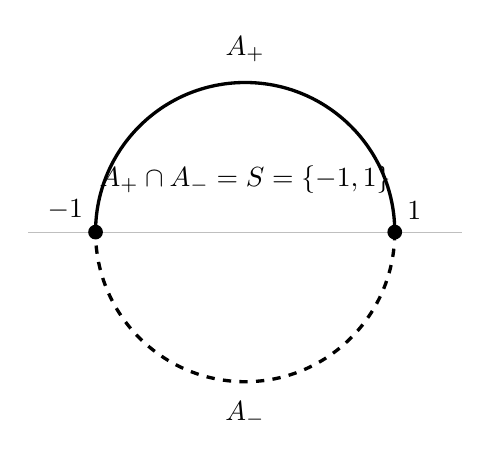
\begin{tikzpicture}[scale=1.9]
  % upper semicircle: solid carrier A_+
  \draw[very thick] (1,0) arc[start angle=0, end angle=180, radius=1];
  \node at (0,1.22) {$A_+$};
  % lower semicircle: dashed carrier A_-
  \draw[very thick, dashed] (1,0) arc[start angle=0, end angle=-180, radius=1];
  \node at (0,-1.22) {$A_-$};
  % faint horizontal axis for orientation
  \draw[gray!50] (-1.45,0) -- (1.45,0);
  % the package points
  \fill (-1,0) circle (1.4pt);
  \node[above left=1pt] at (-1,0) {$-1$};
  \fill (1,0) circle (1.4pt);
  \node[above right=1pt] at (1,0) {$1$};
  % annotation
  \node at (0,0.35) {$A_+\cap A_-=S=\{-1,1\}$};
\end{tikzpicture}
\caption{Two minimal carriers for the package $S=\{-1,1\}$: the upper
semicircle $A_+$ (solid) and the lower semicircle $A_-$ (dashed). Each is an
arc, hence a compact connected full continuum containing $S$, and they meet
only in the package points. A least carrier would be contained in their
intersection $S$, which is disconnected; hence no least carrier exists
(Theorem~\ref{thm:no-least}).}
\label{fig:no-least}
\end{figure}

\subsection{An analytic protected-access collision}\label{subsec:B-collision}

Theorem~\ref{thm:no-least} rules out selecting the carrier by minimization.
The remaining naive rule is completion: accept an arbitrary proposed carrier
and then absorb, monotonically, whatever excess the dynamics pulls back onto
it. The manuscript's Section~6.4 shows that this rule fails as well, and
fails in the most favorable analytic circumstances imaginable: a single
conformal, critical-value-free, degree-one branch of the quadratic map,
acting on an interval. The absorption step erases a protected prime-end
access, and monotonicity then propagates the erasure forever.

We reproduce the analytic setup exactly. Let
\[
f(z)=z^{2},\qquad I=[1,2],\qquad m=\tfrac32,
\]
and let
\begin{equation}\label{eq:B-Q}
Q=\Bigl\{\,z:\bigl|z-\tfrac32\bigr|\le\tfrac12,\ \operatorname{Im}z\ge 0\,\Bigr\}
\end{equation}
be the closed upper half-disk of radius $\tfrac12$ centered at $m$. Set
\[
U^{-}=\bigl\{z:\bigl|z-\tfrac32\bigr|<1\bigr\},
\qquad
U^{+}=f(U^{-}).
\]
The disk $U^{-}$ lies in the half-plane $\operatorname{Re}z>\tfrac12$. Two
consequences follow. First, $0\notin U^{-}$, so $f'(z)=2z\ne 0$ on $U^{-}$
and the critical point of $f$ is outside the domain; since $f(z)=f(w)$ forces
$w=\pm z$, and $U^{-}$ is disjoint from its antipode
$-U^{-}\subset\{\operatorname{Re}z<-\tfrac12\}$, the restriction
\begin{equation}\label{eq:B-branch}
F=f|_{U^{-}}:U^{-}\longrightarrow U^{+}
\end{equation}
is injective, hence a conformal homeomorphism onto $U^{+}$. Second, the
critical value $0=f(0)$ is not in $U^{+}$, so the branch is
critical-value-free. Take
\begin{equation}\label{eq:B-stages}
T_0=I,\qquad T_0'=Q,\qquad T_1=f(I)=[1,4],\qquad T_1'=f(Q).
\end{equation}
Within this branch the stage-$0$ data are the pullbacks of the stage-$1$
data:
\begin{equation}\label{eq:B-pullback}
T_0'=F^{-1}(T_1'),\qquad T_0=F^{-1}(T_1).
\end{equation}
Thus $T_0=I$ is the proposed carrier at stage $0$, and $T_0'=Q$ is the actual
pulled carrier: the completion rule under scrutiny would replace $T_0$ by an
enlargement absorbing the difference. Two pieces of terminology from the
manuscript's completion formalism are needed, and we define them at first
use. The \emph{pulled excess} at stage $0$ is the difference
$X_0=T_0'\setminus T_0$ between the pulled carrier and the proposed carrier.
The \emph{attachment trace} of the excess on the proposed carrier is
\begin{equation}\label{eq:B-trace}
\tau_{T_0}(X_0):=\overline{X_0}^{\,T_0'}\cap T_0,
\end{equation}
where $\overline{X_0}^{\,T_0'}$ denotes the closure of $X_0$ taken in the
actual pulled carrier $T_0'$: the trace records where the excess attaches to
the proposed carrier after closure, not where it meets it as a set.

\begin{proposition}[Quadratic protected-access collision; manuscript Proposition 6.15]\label{prop:access-collision}
In the setup \eqref{eq:B-Q}--\eqref{eq:B-pullback}, the pulled excess has the
single component
\[
X_0=Q\setminus I
\]
with attachment trace
\[
\tau_{T_0}(X_0)=\overline{X_0}^{\,T_0'}\cap T_0=I .
\]
The closure is taken in the actual pulled carrier $T_0'$; in particular, the
trace is not $X_0\cap T_0$, which is empty by the definition of the excess.
The complete one-stage itinerary of the excess is
\[
X_0\longmapsto f(X_0),
\]
through the conformal right-hand branch $F$, with no critical encounter.
Let $p_0^{+}(m)$ denote the upper landing access to $I$ at $m$, represented
by
\[
a_0(t)=m+it,\qquad 0<t\le\tfrac14.
\]
Every compact enlargement $H_0\Subset U^{-}$ with
$I\cup X_0\subset H_0$ erases this access.  Its image enlargement
$F(H_0)$ likewise erases the transported access
$F_*p_0^{+}(m)$, by which we mean the landing access represented by
$F\circ a_0$.
\end{proposition}

\begin{proof}
\emph{The excess and its trace.}
A point of $Q$ lies in $I=[1,2]$ exactly when it is real, so
\[
X_0=Q\setminus I
=\Bigl\{\,z:\bigl|z-\tfrac32\bigr|\le\tfrac12,\ \operatorname{Im}z>0\,\Bigr\}
\]
is the relative upper half-disk with its real diameter removed. It is the
intersection of the closed disk of radius $\tfrac12$ about $m$ with the open
upper half-plane, hence convex, hence connected: the excess has a single
component. Its closure in $\C$ is the entire closed half-disk
$Q$: every $x\in(1,2)$ is the limit of $x+it\in X_0$ as
$t\downarrow0$, while the endpoints are approached, for
$0<\varepsilon\le\tfrac12$, by
$1+\varepsilon+i\varepsilon$ and
$2-\varepsilon+i\varepsilon$, respectively.  As $Q=T_0'$, the closure of
$X_0$ in $T_0'$ is all of $Q$,
and therefore
\[
\tau_{T_0}(X_0)=\overline{X_0}^{\,T_0'}\cap T_0=Q\cap I=I:
\]
the excess attaches to the proposed carrier along the entire interval, even
though $X_0\cap T_0=\varnothing$ by construction. This is the reason the
completion formalism must work with attachment traces rather than
intersections: the naive intersection sees nothing, while the closure sees an
attachment along all of $I$.

\emph{The itinerary.}
Since $0\notin U^{-}$, we have $F'(z)=2z\ne 0$ throughout $U^{-}$, and the
selected branch avoids the critical value $0\notin U^{+}$. The itinerary of
the excess therefore consists of the single right-sheet, degree-one step
$X_0\mapsto f(X_0)$ with no critical encounter.
There is no hidden multivalence, folding, or critical intrusion anywhere in
the example.

\emph{Erasure of the protected access.}
The access $p_0^{+}(m)$ is the access to $I$ at the interior point $m$ from
the upper side, represented by $a_0$, which lies in
$U^{-}\setminus I$ and lands at $m$.  Let
$H_0\Subset U^{-}$ be compact and contain $X_0\cup I=Q$.  The set $Q$ contains an
upper relative half-neighborhood of $m$: the set
\[
\Bigl\{\,z:\bigl|z-\tfrac32\bigr|<\tfrac12,\ \operatorname{Im}z\ge 0\,\Bigr\}
\subset Q
\]
is a neighborhood of $m$ in the closed upper half-plane. Consequently, any
curve in $U^{-}$ landing at $m$ from the upper side---that is, eventually
in the upper component of a sufficiently small disk about $m$ with $I$
removed---eventually lies in this half-neighborhood, hence in $Q\subset H_0$.
No curve in the complement $U^{-}\setminus H_0$ can therefore land at $m$ from the upper
side: the access $p_0^{+}(m)$ no longer exists as an access from the
complement of $H_0$.  Any further enlargement still contains $Q$ and
cannot restore that access.

\emph{Transport to stage $1$.}
The branch $F$ of \eqref{eq:B-branch} is a conformal homeomorphism of
$U^{-}$ onto $U^{+}$ carrying $I$ to $T_1=[1,4]$, $Q$ to $T_1'$, $X_0$ to the
stage-$1$ excess $T_1'\setminus T_1$, and the representing curve $m+it$ to a
curve in $U^{+}\setminus T_1$ landing at $f(m)=\tfrac94$ from the
$F$-selected side.  The compact image $F(H_0)$ contains
$F(Q)=T_1'$.  A homeomorphism of the localization carries complement
curves to complement curves, so the same argument applied to these image data
erases the transported access $F_{*}p_0^{+}(m)$ at stage $1$. Conformality
thus transports the identical conclusion to stage $1$, as claimed.
\end{proof}

\begin{figure}[ht]
\centering
\begin{tikzpicture}[scale=2.6]
  % localization disk U^- (dashed)
  \draw[dashed] (1.5,0) circle[radius=1];
  \node at (2.28,0.82) {$U^{-}$};
  % real axis
  \draw[->,gray] (0.25,0) -- (2.85,0) node[right,black] {$\mathbb{R}$};
  % excess half-disk Q (shaded)
  \fill[gray!30] (2,0) arc[start angle=0, end angle=180, radius=0.5] -- cycle;
  \draw (2,0) arc[start angle=0, end angle=180, radius=0.5];
  \node at (1.72,0.3) {$Q$};
  % proposed carrier I = [1,2]
  \draw[very thick] (1,0) -- (2,0);
  \draw (1,0.025) -- (1,-0.025) node[below] {$1$};
  \draw (2,0.025) -- (2,-0.025) node[below] {$2$};
  \node[below] at (1.25,-0.05) {$I$};
  % marked point m
  \fill (1.5,0) circle (0.8pt);
  \node[below] at (1.5,-0.045) {$m=\tfrac32$};
  % protected access arrow from above, along m + it
  \draw[-{Stealth[length=2mm]},very thick] (1.5,0.92) -- (1.5,0.035);
  \node[right] at (1.53,0.6) {$p_0^{+}(m)\colon\ m+it$};
  % annotation: the collar at m is inside Q
  \node[align=left,right] at (2.15,0.38) {upper collar at $m$\\ lies inside $Q$};
  \draw[-{Stealth[length=1.6mm]},gray] (2.14,0.33) -- (1.62,0.14);
\end{tikzpicture}
\caption{The quadratic protected-access collision
(Proposition~\ref{prop:access-collision}). The proposed carrier is the
interval $I=[1,2]$ (thick); the pulled carrier is the closed upper half-disk
$Q$ (shaded) of radius $\tfrac12$ about $m=\tfrac32$, inside the localization
disk $U^{-}$ (dashed) on which $f(z)=z^{2}$ restricts to a conformal
homeomorphism. The protected upper access $p_0^{+}(m)$, represented by the
vertical segment $m+it$, must traverse $Q$: absorbing the excess
$X_0=Q\setminus I$ forces the carrier to contain the entire upper collar at
$m$ and erases the access.}
\label{fig:access-collision}
\end{figure}

\subsection{What the obstructions force}\label{subsec:B-moral}

The two obstructions are complementary and together close off every naive
route. Theorem~\ref{thm:no-least} shows that the carrier cannot be
\emph{selected} canonically: there is no least connected full hull, even for
two points with identity dynamics.  Minimal carriers may exist, as the two
semicircles in the proof show, but they need not be unique and neither is
least; thus ``the minimal carrier'' does not specify an object.
Proposition~\ref{prop:access-collision} shows that the carrier cannot be
\emph{completed} blindly either: the very first monotone absorption of a
pulled excess can erase a protected prime-end access, and monotonicity then
makes the loss irreversible at every later stage of the enlargement, as well
as at the conformally transported stage.

The second obstruction is the sharper of the two, because of what it does
\emph{not} involve. In the manuscript's collision bookkeeping \cite{MWman},
which records sheet mergers, critical intrusions, obstacle collisions, access
identifications, and localization escapes in the order
$(\chi_{\mathrm{sheet}},\chi_{\mathrm{crit}},\chi_{\mathrm{obs}},
\chi_{\mathrm{access}},\chi_{\mathrm{loc}})$, the collision tuple of the
completed enlargement in this example is
\[
\bigl(\varnothing,\ \varnothing,\ \varnothing,\
\{p_0^{+}(m),\,F_{*}p_0^{+}(m)\},\ \varnothing\bigr):
\]
every coordinate vanishes except the access coordinate. The
branch is conformal, degree one, and critical-value-free; there is no sheet
merger, no obstacle, and no localization escape. Consequently no amount of
critical-point bookkeeping---however carefully one tracks critical points,
critical values, or degrees---can detect, let alone excuse, the collision.
Access protection is invisible to critical data and must be carried as
explicit data of its own, with its own survival theorem.

This is exactly what the remainder of the paper provides. The certificate
formalism of Section~\ref{sec:certificates} records the protected accesses as
prime-end crosscut chains \cite{Pom92} with pairwise disjoint relative
terminal collar tails, together with free-port arcs carrying singleton attachment traces
and a ribbon tree with declared sides; Theorem~\ref{thm:realization} then
realizes any such certificate by an actual compact connected full carrier in
which every protected chain survives with unchanged cyclic order. The
selection ambiguity of Theorem~\ref{thm:no-least} is resolved not by
minimization but by the certificate itself: the connector system, its access
class, and its routing are supplied as data, and the exact free-component
criterion of Section~\ref{sec:criterion} determines precisely when such data
can be supplied at all.
